
\begin{multicols}{2}
 ние приводится к виду $4\cos y=-3\cos 3y$, или $\cos y = -3\cos 3y - 3 \cos y = -6\cos y * \cos 2y$, \\ \textbf{2. 9109}.\textit{Указание}. Пусть A=$xyzt$, где $x$, $y$, $z$, $t$ $-$ цифры. Из условия после преобразований получим уравнение $111(x-t)+10(y-z)$=10, откуда $x=t$, $y-z=1$.\\
\textbf{3.} ($3;+\infty)$ при $a\leq 2$;\\
$(2; a) \cup (3;+\infty)$ при $2<a\leq 3$;\\
$(2;3) \cup (a; +\infty)$ при $a>3$\\
\textit{Указание.} Исходное неравенство равносиль-\linebreak но совокупности двух систем:\\
\begin{fleqn}
\begin{equation*}
	\left\{
		\begin{array}{lcl}
		x-a>0,\\
		\log_{3}(x-2)>0
		\end{array}
	\right.
	\quad\text{или}\quad
	\left\{
		\begin{array}{lcl}
		x-a<0,\\
		\log_{3}(x-2)<0.
		\end{array}
	\right.
\end{equation*}
\end{fleqn}
\textbf{4.}
\large{$\dfrac{d^{2} \sin\phi \sin\alpha (1+2\cos 2\phi)}{8\cos^{3}\phi}$}
\large{×}\\ \large{×} \large{$\sqrt{4 \cos^{2}\alpha  \cos^{2}\phi + \sin^{2}\alpha (1-2\cos 2\phi)^{2}}$}\\
при $0 < \phi < \pi / 4$;\\
\large{$\dfrac{1}{4}d^{2}\sin 2\alpha \sin 2\phi \dfrac{\sqrt{4\cos^{2}\phi+\tg^{2}\alpha(2\sin \phi - \cos 2\phi)^{2}}}{2\sin\phi-\cos 2\phi}$}\\
\normalsize{при $\pi /4 \leq \phi < \pi /2$}\\
\textit{Указание}. Пусть $O$ - центр описанной около\\ треугольника $ABC$ окружности, $O_{1}$ $-$ точка пересечения
высот равного ему треугольника $A_{1}B_{1}C_{1}$ (рис. 5). Если 0<$\phi$<$\pi$/4, треугольник
$ABC$ остроугольный и точки $O$ и $O_{1}$ лежат внутри треугольников $ABC$ и $A_{1}B_{1}C_{1}$ соответственно, так что в этом случае сечение является трапецией (рис. 6). При $\pi/4\leq\phi<\pi/2$ треугольники $ABC$ и $A_{1}B_{1}C_{1}$
либо прямоугольные (при $\phi=\pi/4$), либо тупоугольные, а сечение будет треугольником (рис. 7).\\
В первом случае $AB$=$d\sin\alpha$, $BB_{1}$=$d\cos\alpha$. Пусть $O_{2} -$ точка пересечения высот треугольника $ABC$ (рис. 8). Тогда $BO$=$AB/(2\cos\phi)$, $BO_{2}$=$BC\times\cos 2\phi/\cos\phi$ и $OO_{2}$=$|BO$-$BO_{2}|=
d\sin\alpha|1-2\cos 2\phi|/(2\cos\phi)$. Высоту $OO_{1}$ трапеции находим из соотношения \\
$$OO_{1}^{2}=OO_{2}^{2}+BB_{1}^{2}.$$\\
Для вычисления оснований трапеции - отрезков $MN$ и $M_{1}N_{1}$ - воспользуйтесь подобием соответствующих треугольников: \\
$$MN=AC\cdot\dfrac{BO}{BD};  M_{1}N_{1}=AC\cdot\dfrac{BO_{2}}{BD}.$$\\
Если $\pi/4\leq\phi<\pi/2$, сечение $-$ треугольник с основанием, равным $AC=2d\sin\alpha\sin\phi$ и высотой $KL$.\\
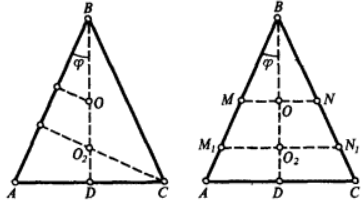
\includegraphics[scale=0.8]{ris8.png}\\
\textit{Рис. 8.}\\
\columnbreak
\\
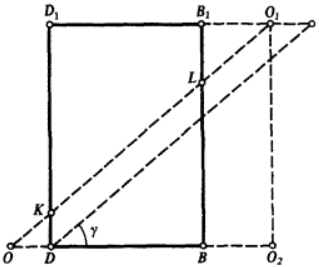
\includegraphics[scale=0.8]{pictures/ris9.png}\\
\textit{Рис. 9.}\\\\
При вычислении $KL$ нужно, как и раньше, найти $OO_{2}=O_{2}D+OB-BD$ (рис. 9), заметить, что $KL=BD/\cos\gamma$, где $\gamma -$ угол наклона секущей плоскти к плоскости основания и воспользоваться тем, что $\tg\gamma=B_{1}B/OO_{2}.$\\
\large{\textit{Вариант 2}}
\\
\textbf{1}. $\dfrac{\pi}{4}(4k+1)$; $-\dfrac{\pi}{4}+(-1)^{k}\arcsin\dfrac{4-\sqrt{17}}{\sqrt{2}}+\pi k, k \in Z$.\\
\textbf{2}. 60 ч.\\
\textbf{3}. $x_{1}=-(c+63); x_{2}=1-c$. Оба корня положительны при $c<-63$.\\
\textbf{4}. Если $0<\gamma\leq\arccos\dfrac{1}{3}$, имеются два существенно различных случая: $R_{1}=\dfrac{h}{2}\sqrt{\dfrac{3\cos\gamma-1}{\cos\gamma}}$ (сечение параллельно плоскости основания) и $R_{2}=h\sqrt{2}\dfrac{\ctg\gamma\cdot\tg\gamma/2 }{\sqrt{2+\ctg^{2}\gamma}}$ (сечение параллельно боковой грани). Если $\arccos\dfrac{1}{3}<\gamma<\pi/2$, остаются только сечения, параллельные боковым граням, при этом $R=R_{2}$.\\
\textbf{Физика}\\
Билет 1\\
\textbf{1}. Полное ускорение $\vec{a}$ складывается из нормального $\vec{a_{n}}$ и тангенциального $\vec{a_{\tau}}$:
\vspace{-0.1cm}
$$a=\sqrt{a_{n}^{2}+a_{\tau}^{2}}.$$
Нормальное ускорение равно $a_{n}=\upsilon^{2}/R$, а скорость тела $\upsilon$ при постоянном тангенциальном ускорении линейно растет со временем: $\upsilon=a_{\tau}t.$ В результате получаем \vspace{-0.35cm}
$$a=\sqrt{((a_{\tau}t)^{2}/R)^{2}+a_{\tau}^{2}}=a_{\tau}\sqrt{1+(a_{\tau}t^{2}/R)^{2}}.$$
\textbf{2}. Средняя энергия атома аргона $\overline{E}$ связана с температурой $T$ соотношением $\overline{E}=\sfrac{3}{2}kT$, где $k -$ постоянная Больцмана. Температуру найдем из уравнения Клайперона-Менделеева: $T=pV/(\nu R)$. Тогда $\overline{E}=\sfrac{3}{2}kpV/(\nu R)=\sfrac{3}{2}pV/(\nu N_{A}) = 1,2 \cdot 10^{-23}$ Дж, где $N_{A} = 6 \cdot 10^23$ моль$^{-1}$ - число Авогадро.
\begin{flushright}
	\Huge{\textbf{77}}
\end{flushright}
\end{multicols}
\newpage
\begin{multicols}{2}
	\textbf{3}. Потенциал шарика возрастает до тех пор, пока кингетическая энергия самых быстрых вылетающих из него фотоэлектронов достаточна для того, чтобы они смогли преодолеть возникающий задерживающий потенциал и удалиться от шарика на бесконечно большое расстояние. Поэтому уравнение Эйнштейна для фотоэффейта запишется в виде
$$hc/\lambda = A + e\phi_{max}$$
откуда находим искомую работу выхода $A$:
$$A=hc/\lambda-e\phi_{max}=4,36 \text{ эВ.}$$ 
\textbf{4}. Поскольку сила, действующая на протон со стороны магнитного поля, не изменяет величину скорости $\upsilon$, а начальная скорость протона равна нулю, закон сохранения энергии - для момента, когда протон находится в точке $A$, и для начального момента - запишется в виде
$$m\upsilon^{2}/2-eEh=0.$$
Второй закон Ньютона для протона в точке $A$, в проекциях на ось $Y$, выглядит так:
$$-ma=eE-e\upsilon B.$$
Таким образом, ускорение протона равно
$$a=(e/m)(B\sqrt{2(e/m)Eh}-E)=10^{12} \text{ м/с$^{2}$.}$$
\textit{Билет 2}\\
\textbf{1}. На рисунке (см. рис. 2 в статье) представлены графики изобарны процессов. Давление газа в состоянии 1 мекньше, чем в состоянии 4.\\ \textbf{2}. На частицу в магнитном поле действует сила Лоренца $F=|q|\upsilon B$, сообщающая ей центростремительное ускорение $a=\upsilon^{2}/R=F/m=|q|\upsilon B/m$. Отсюда
$$|q|=m\upsilon/(BR).$$
Правило нахождения направления силы $\vec{F}$ дает ответ на вопрос о знаке заряда - он отрицательный.\\
\textbf{3}. Ускорение системы, состоящзей из нити и обоих тел, равно 
$$a=F/(m_{1}+m_{2}+m).$$
Тело $A$ движется под действием силы натяжения нити в точке соединения с этим телом, поэтому 
$$T_{A}=m_{2}a=Fm_{2}/(m_{1}+m_{2}+m).$$
Ускорение тела $B$ обсуловлено действием на него силы $\vec{F}$ и силы натяжения нити в точке соединения с ним:
$$m_{1}a=F-T_{B},$$
следовательно, $$T_{B}=F-m_{1}a=F(m_{2}+m)/(m_{1}+m_{2}+m).$$
\textbf{4}. Пользуясь свойством обратимости хода лучей, точку $S$ можно рассматривать как мнимое изображение. Тогда формула линзы запишется в виде
$$\frac{1}{d}-\frac{1}{l}=D,$$ где $d$ - расстояние от линзы до точки пересечения лучей, преломившихся в линзе. Отсюда $$d=l/(1+Dl)=13,6 \text{см.}$$\\
\begin{flushleft}
	\Huge{\textbf{78}}
\end{flushleft}
\columnbreak
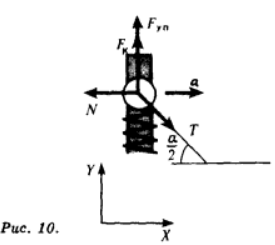
\includegraphics[scale=0.9]{ris10.png}
\\
\textit{Билет 3}\\
\textbf{1}. Уравнение движения тела, брошенного под углом к горизонту, имеет вид
\vspace{-0.3cm}
$$\vec{r}=\vec{r_{0}}+\vec{v_{0}}t-\vec{g}t^{2}/2,$$
где $\vec{r} -$ радиус-вектор тела в произвольный момент движения t, $\vec{r_{0}} - $ начальный радиус-вектор, $\vec{v_{0}} - $ начальная скорость тела.\\
\textbf{2}. Внутренняя энергия $\nu$ молей одноатомного газа связана с его температурой соотношением
$U=\sfrac{3}{2}\nu RT.$\\\\
Теперь из уравнения Клапейрона-Менделеева легко найти давление газа:
\vspace{-0.3cm}
$$p=\nu RT/V=2U(3V)=1 \text{атм.}$$
\textbf{3}. Лучи, преломившиеся в линзе и отразившиеся от зеркала, вновь преломляются в линзе. Поэтому оптическая система ``линза+зеркало'' равна удвоенной оптической силе линзы, а уравнение этой системы имеет вид
\vspace{-0.3cm}
$$\frac{1}{d}+\frac{1}{f}=\frac{2}{F}.$$
Отсюда получаем $f=Fd/(2d-F)=-20 $ см.\\
Изображение мнимое и находится на расстоянии 20 см от линзы.\\
\textbf{4}. Запишем второй закон Ньютона для системы в целом:
$m\vec{a}=\vec{F}$, а также для одной из муфточек (рис.10):
$m_{M}\vec{a}=\vec{T}+\vec{F_{уп}}+\vec{N}+\vec{F_{к}},$
где $m_{M} - $ масса муфточки, $\vec{T} - $ сила натяжения нити, $\vec{F_{уп}}- $ сила упругости пружины, $\vec{N}- $ сила нормальной реакции стержня, $\vec{F_{к}}- $ сила кулоновского взаимодействия муфточек. Запишем эти уравнения в проекциях на оси $X$ и $Y$ соответственно:
$ma=F,$
\vspace{-0.3cm}
$$0=-T\sin(\alpha/2)+k(l_{0}-l)+q^{2}/(4\pi\varepsilon_{0}l^{2}),$$
где $l - $ расстояние между муфточками. Заметим также, что силы $T$ и $F$ связаны соотношением
$$F=2T\cos(\alpha/2),$$
а величина $l$ может быть выражена через $l_{0}$:
\vspace{-0.3cm}
$$l=l_{0}\sin(\alpha/2).$$
\end{multicols}
\newpage
\begin{center}
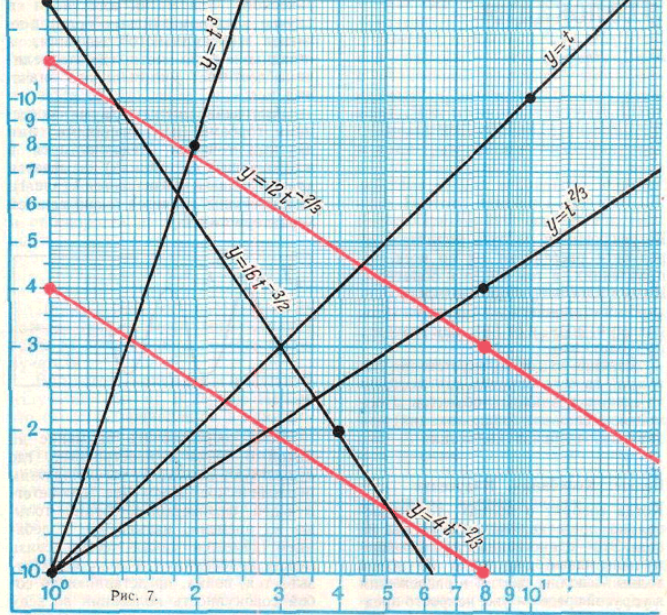
\includegraphics[scale=0.9]{ris11.png}
	\begin{minipage}{0.25\textwidth}
  		\textit{Замечание}. Во всей промышленной продукции группа $A$ в 1913 году составлялс 35,1\%, а в 1970 году 74,8\%.
	\begin{flushright}
		\textit{Таблица}
	\end{flushright}
	\begin{tabular}{|r |r| r|}
		\hline
		Год & Группа & Группа\\
		& A &B\\
		\hline
		1913&100&100\\
		1917&81&67\\
		1928&155&120\\
		1932&424&187\\
		1937&1013&373\\
		1940&1340&460\\
		1945&1504&273\\
		1950&2746&566\\
		1955&5223&996\\
		1960&8936&1498\\
		1965&14156&2032\\
		1970&21359&3281
	\end{tabular}
	\end{minipage}
\hfill
	\begin{minipage}{0.65\textwidth}
  		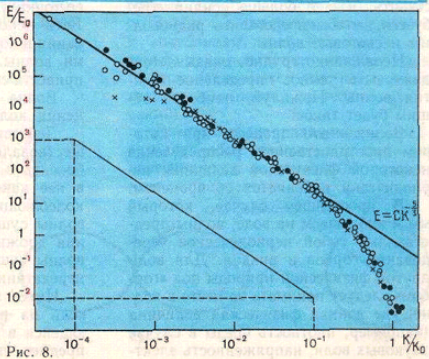
\includegraphics{ris12.png}
		\\\\\\
		\begin{flushright}
			\large{\textbf{7}}
		\end{flushright}
	\end{minipage}
\end{center} 